% Options for packages loaded elsewhere
% Options for packages loaded elsewhere
\PassOptionsToPackage{unicode}{hyperref}
\PassOptionsToPackage{hyphens}{url}
\PassOptionsToPackage{dvipsnames,svgnames,x11names}{xcolor}
%
\documentclass[
  english,
  10pt,
  letterpaper,
  DIV=11,
  numbers=noendperiod]{scrartcl}
\usepackage{xcolor}
\usepackage[margin=1in]{geometry}
\usepackage{amsmath,amssymb}
\setcounter{secnumdepth}{5}
\usepackage{iftex}
\ifPDFTeX
  \usepackage[T1]{fontenc}
  \usepackage[utf8]{inputenc}
  \usepackage{textcomp} % provide euro and other symbols
\else % if luatex or xetex
  \usepackage{unicode-math} % this also loads fontspec
  \defaultfontfeatures{Scale=MatchLowercase}
  \defaultfontfeatures[\rmfamily]{Ligatures=TeX,Scale=1}
\fi
\usepackage{lmodern}
\ifPDFTeX\else
  % xetex/luatex font selection
\fi
% Use upquote if available, for straight quotes in verbatim environments
\IfFileExists{upquote.sty}{\usepackage{upquote}}{}
\IfFileExists{microtype.sty}{% use microtype if available
  \usepackage[]{microtype}
  \UseMicrotypeSet[protrusion]{basicmath} % disable protrusion for tt fonts
}{}
\makeatletter
\@ifundefined{KOMAClassName}{% if non-KOMA class
  \IfFileExists{parskip.sty}{%
    \usepackage{parskip}
  }{% else
    \setlength{\parindent}{0pt}
    \setlength{\parskip}{6pt plus 2pt minus 1pt}}
}{% if KOMA class
  \KOMAoptions{parskip=half}}
\makeatother
% Make \paragraph and \subparagraph free-standing
\makeatletter
\ifx\paragraph\undefined\else
  \let\oldparagraph\paragraph
  \renewcommand{\paragraph}{
    \@ifstar
      \xxxParagraphStar
      \xxxParagraphNoStar
  }
  \newcommand{\xxxParagraphStar}[1]{\oldparagraph*{#1}\mbox{}}
  \newcommand{\xxxParagraphNoStar}[1]{\oldparagraph{#1}\mbox{}}
\fi
\ifx\subparagraph\undefined\else
  \let\oldsubparagraph\subparagraph
  \renewcommand{\subparagraph}{
    \@ifstar
      \xxxSubParagraphStar
      \xxxSubParagraphNoStar
  }
  \newcommand{\xxxSubParagraphStar}[1]{\oldsubparagraph*{#1}\mbox{}}
  \newcommand{\xxxSubParagraphNoStar}[1]{\oldsubparagraph{#1}\mbox{}}
\fi
\makeatother


\usepackage{longtable,booktabs,array}
\newcounter{none} % for unnumbered tables
\usepackage{calc} % for calculating minipage widths
% Correct order of tables after \paragraph or \subparagraph
\usepackage{etoolbox}
\makeatletter
\patchcmd\longtable{\par}{\if@noskipsec\mbox{}\fi\par}{}{}
\makeatother
% Allow footnotes in longtable head/foot
\IfFileExists{footnotehyper.sty}{\usepackage{footnotehyper}}{\usepackage{footnote}}
\makesavenoteenv{longtable}
\usepackage{graphicx}
\makeatletter
\newsavebox\pandoc@box
\newcommand*\pandocbounded[1]{% scales image to fit in text height/width
  \sbox\pandoc@box{#1}%
  \Gscale@div\@tempa{\textheight}{\dimexpr\ht\pandoc@box+\dp\pandoc@box\relax}%
  \Gscale@div\@tempb{\linewidth}{\wd\pandoc@box}%
  \ifdim\@tempb\p@<\@tempa\p@\let\@tempa\@tempb\fi% select the smaller of both
  \ifdim\@tempa\p@<\p@\scalebox{\@tempa}{\usebox\pandoc@box}%
  \else\usebox{\pandoc@box}%
  \fi%
}
% Set default figure placement to htbp
\def\fps@figure{htbp}
\makeatother


% definitions for citeproc citations
\NewDocumentCommand\citeproctext{}{}
\NewDocumentCommand\citeproc{mm}{%
  \begingroup\def\citeproctext{#2}\cite{#1}\endgroup}
\makeatletter
 % allow citations to break across lines
 \let\@cite@ofmt\@firstofone
 % avoid brackets around text for \cite:
 \def\@biblabel#1{}
 \def\@cite#1#2{{#1\if@tempswa , #2\fi}}
\makeatother
\newlength{\cslhangindent}
\setlength{\cslhangindent}{1.5em}
\newlength{\csllabelwidth}
\setlength{\csllabelwidth}{3em}
\newenvironment{CSLReferences}[2] % #1 hanging-indent, #2 entry-spacing
 {\begin{list}{}{%
  \setlength{\itemindent}{0pt}
  \setlength{\leftmargin}{0pt}
  \setlength{\parsep}{0pt}
  % turn on hanging indent if param 1 is 1
  \ifodd #1
   \setlength{\leftmargin}{\cslhangindent}
   \setlength{\itemindent}{-1\cslhangindent}
  \fi
  % set entry spacing
  \setlength{\itemsep}{#2\baselineskip}}}
 {\end{list}}
\usepackage{calc}
\newcommand{\CSLBlock}[1]{\hfill\break\parbox[t]{\linewidth}{\strut\ignorespaces#1\strut}}
\newcommand{\CSLLeftMargin}[1]{\parbox[t]{\csllabelwidth}{\strut#1\strut}}
\newcommand{\CSLRightInline}[1]{\parbox[t]{\linewidth - \csllabelwidth}{\strut#1\strut}}
\newcommand{\CSLIndent}[1]{\hspace{\cslhangindent}#1}

\ifLuaTeX
\usepackage[bidi=basic,shorthands=off]{babel}
\else
\usepackage[bidi=default,shorthands=off]{babel}
\fi
\ifLuaTeX
  \usepackage{selnolig} % disable illegal ligatures
\fi


\setlength{\emergencystretch}{3em} % prevent overfull lines

\providecommand{\tightlist}{%
  \setlength{\itemsep}{0pt}\setlength{\parskip}{0pt}}



 


\KOMAoption{captions}{tableheading}
\makeatletter
\@ifpackageloaded{caption}{}{\usepackage{caption}}
\AtBeginDocument{%
\ifdefined\contentsname
  \renewcommand*\contentsname{Table of contents}
\else
  \newcommand\contentsname{Table of contents}
\fi
\ifdefined\listfigurename
  \renewcommand*\listfigurename{List of Figures}
\else
  \newcommand\listfigurename{List of Figures}
\fi
\ifdefined\listtablename
  \renewcommand*\listtablename{List of Tables}
\else
  \newcommand\listtablename{List of Tables}
\fi
\ifdefined\figurename
  \renewcommand*\figurename{Figure}
\else
  \newcommand\figurename{Figure}
\fi
\ifdefined\tablename
  \renewcommand*\tablename{Table}
\else
  \newcommand\tablename{Table}
\fi
}
\@ifpackageloaded{float}{}{\usepackage{float}}
\floatstyle{ruled}
\@ifundefined{c@chapter}{\newfloat{codelisting}{h}{lop}}{\newfloat{codelisting}{h}{lop}[chapter]}
\floatname{codelisting}{Listing}
\newcommand*\listoflistings{\listof{codelisting}{List of Listings}}
\usepackage{amsthm}
\theoremstyle{plain}
\newtheorem{theorem}{Theorem}[section]
\theoremstyle{plain}
\newtheorem{proposition}{Proposition}[section]
\theoremstyle{plain}
\newtheorem{lemma}{Lemma}[section]
\theoremstyle{plain}
\newtheorem{corollary}{Corollary}[section]
\theoremstyle{definition}
\newtheorem{definition}{Definition}[section]
\theoremstyle{remark}
\AtBeginDocument{\renewcommand*{\proofname}{Proof}}
\newtheorem*{remark}{Remark}
\newtheorem*{solution}{Solution}
\newtheorem{refremark}{Remark}[section]
\newtheorem{refsolution}{Solution}[section]
\makeatother
\makeatletter
\makeatother
\makeatletter
\@ifpackageloaded{caption}{}{\usepackage{caption}}
\@ifpackageloaded{subcaption}{}{\usepackage{subcaption}}
\makeatother
\usepackage{bookmark}
\IfFileExists{xurl.sty}{\usepackage{xurl}}{} % add URL line breaks if available
\urlstyle{same}
% fallback for those not using the hyperref driver hyperxmp:
\makeatletter
\@ifundefined{xmpquote}{\newcommand{\xmpquote}[1]{#1}}{}
\makeatother
\hypersetup{
  pdftitle={Exact Bounded Correlation},
  pdfauthor={Complex--Itô Random-Walk Research Project},
  pdflang={en},
  pdfkeywords={\xmpquote{stochastic correlation}, \xmpquote{one-phase
Euler coordinates}, \xmpquote{barrier options}, \xmpquote{first
passage}, \xmpquote{Dambis--Dubins--Schwarz}, \xmpquote{Feynman--Kac}, \xmpquote{occupation
time}, \xmpquote{Ornstein--Uhlenbeck}, \xmpquote{Bachelier model}},
  colorlinks=true,
  linkcolor={blue},
  filecolor={Maroon},
  citecolor={Blue},
  urlcolor={Blue},
  pdfcreator={LaTeX via pandoc}}


\title{Exact Bounded Correlation}
\usepackage{etoolbox}
\makeatletter
\providecommand{\subtitle}[1]{% add subtitle to \maketitle
  \apptocmd{\@title}{\par {\large #1 \par}}{}{}
}
\makeatother
\subtitle{One-Phase Euler Coordinates for Stochastic Correlation,
Derivative Pricing, and Joint Barriers}
\author{Complex--Itô Random-Walk Research Project}
\date{July 27, 2026}
\begin{document}
\maketitle
\begin{abstract}
We construct a stochastic-correlation framework in which the correlation
state is the sine of the one-phase Euler phase of a scalar Gaussian
factor: \(\rho_t=X_t/\sqrt{X_t^2+c^2}\) with
\(X_t=x_0+\mu t+\sigma W_t\). Because the map is a monotone conjugacy,
the framework inherits exact laws that no tractable competitor possesses
jointly: a closed-form finite-time transition density;
reflection-principle first-passage laws for correlation barriers; and
exact prices for correlation derivatives --- digitals, one-touches paid
at expiry and at hit (a new closed form via a completing-the-square
identity), and discretely monitored range accruals. For two assets
driven by Brownian motions correlated through \(\rho_t\), with the
correlation driver independent of the asset drivers, the
Dambis--Dubins--Schwarz theorem reduces every linear combination of the
assets --- spreads, baskets --- to Brownian motion with a deterministic
variance clock, collapsing joint barrier pricing to a scalar functional
of the correlation path. The full law of that clock is computed
deterministically by a Feynman--Kac resolvent and a Fourier series (the
clock's support is bounded), verified against exact-skeleton Monte
Carlo. The same resolvent prices continuous corridor occupation
derivatives after an explicit atom separation, reproducing Lévy's
arcsine law as a parameter-free anchor. Replacing the Brownian driver by
an Ornstein--Uhlenbeck driver yields a mean-reverting correlation state
with exact stationary density, and we prove the
stationarity--tractability classification: static laws and the clock
reduction survive, while closed-form first-passage laws are surrendered
to the resolvent. All claims are verified by unit tests and reproducible
notebooks; economic costs (non-stationarity under the Brownian driver,
polynomial boundary tails, exclusion of leverage) are stated explicitly.
\end{abstract}

\renewcommand*\contentsname{Table of contents}
{
\setcounter{tocdepth}{2}
\tableofcontents
}

\textbf{Mathematics Subject Classification (2020):} 60H10, 60J60, 60J65,
91G20, 91G60.

\textbf{JEL classification:} C02, C63, G12, G13.

\section{Introduction}\label{sec-introduction}

Correlation is the canonical bounded state variable of multi-asset
finance, and it is empirically stochastic (Teng et al. 2016; Driessen et
al. 2009). The modeling question is thirty years old and the answers
split into two families, both with structural defects for pricing.
Bounded \emph{intrinsic} diffusions --- the Jacobi process of van
Emmerich (Emmerich 2006; Ackerer et al. 2018) --- are mean-reverting but
have no closed-form transition density, so likelihoods and prices need
spectral expansions. \emph{Transform} models --- correlation as a
bounded function of a Gaussian factor, as in the hyperbolic-tangent
model of Teng, Ehrhardt, and Günther (Teng et al. 2016) --- have exact
marginals by change of variables, but the transform in use has never
been given the path-level laws that exotic pricing consumes: barrier and
one-touch structures under stochastic correlation are handled by
approximation (Higgins 2014), and the first-passage problems of the
underlying drivers are unsolved in closed form outside the Brownian case
(Ricciardi and Sato 1988; Alili et al. 2005).

This paper closes that gap for one particular transform --- the one
whose path-level laws \emph{are} closed form. The correlation state is

\[
\rho_t=\sin\theta_t=\frac{X_t}{\sqrt{X_t^{2}+c^{2}}},\qquad
\theta_t=\arctan(X_t/c),\qquad X_t=x_0+\mu t+\sigma W_t,
\]

the sine of the \emph{one-phase Euler phase} of the companion paper
(Complex--Itô Random-Walk Research Project 2026), where \(\theta_t\) was
proved to be the unique lossless phase coordinate of an affine complex
Brownian process. The map \(x\mapsto x/\sqrt{x^{2}+c^{2}}\) is a smooth
monotone conjugacy between the real line and \((-1,1)\); every path
property of \(X\) therefore transfers to \(\rho\), and the Brownian
driver's reflection principle becomes exact first-passage law for
correlation barriers. No Jacobi, tanh-transformed-OU, or circular model
has this, because their drivers' first-passage problems admit no
reflection principle.

The contributions, each verified in the companion notebook (Complex--Itô
Random-Walk Research Project 2026, companion notebook therein) and the
reproducibility material of this paper, are:

\begin{enumerate}
\def\labelenumi{\arabic{enumi}.}
\tightlist
\item
  \textbf{Exact kernels} (Section~\ref{sec-coordinate},
  Section~\ref{sec-firstpassage}): the finite-time transition density,
  the first-passage CDF and density, the perpetual hitting probability,
  and the two-sided band-exit law of \(\rho_t\), all in terms of the
  Gaussian CDF; plus invariance of the entire class under Girsanov
  measure changes with constant correlation risk premium.
\item
  \textbf{Exact correlation derivatives}
  (Section~\ref{sec-derivatives}): digital, one-touch paid at expiry,
  one-touch paid at hit --- the last a new closed form obtained by
  completing the square in the inverse-Gaussian density --- and
  discretely monitored range accruals.
\item
  \textbf{The variance-clock reduction} (Section~\ref{sec-reduction}):
  for two Bachelier assets correlated through \(\rho_t\), any linear
  combination is, conditionally on the correlation path, Brownian motion
  with a deterministic clock. Joint barrier pricing collapses from three
  drivers to one scalar functional, with a sign theorem: correlation
  risk misprices spread and basket barriers in \emph{opposite}
  directions.
\item
  \textbf{The full clock law} (Section~\ref{sec-fk}): the clock's
  bounded support turns its Feynman--Kac characteristic function into a
  Fourier series, giving deterministic prices with two monitored
  discretization errors, statistically indistinguishable from exact
  simulation (\(|z|<1\) in all reported configurations).
\item
  \textbf{Corridor occupation} (Section~\ref{sec-corridor}): the same
  resolvent with an indicator potential, after explicit separation of
  the never-exit atom, prices continuous corridor digitals and calls;
  the driftless half-line case reproduces Lévy's arcsine law to
  \(5\times10^{-4}\).
\item
  \textbf{The OU driver and the classification} (Section~\ref{sec-ou}):
  an Ornstein--Uhlenbeck driver makes the correlation state
  mean-reverting with exact stationary density; we classify precisely
  what is kept (static laws, clock reduction, resolvent machinery) and
  what is surrendered (reflection-principle hitting laws), and verify
  the \(\kappa\to0^{+}\) degeneration into the Brownian results.
\end{enumerate}

Section~\ref{sec-related} states the novelty boundary: we do not claim
the transform itself (bounded functions of Gaussian factors are
established (Emmerich 2006; Teng et al. 2016)), nor a new correlation
model in the empirical sense; the claim is the exact path-level and
pricing content of this coordinate, which the audited literature does
not contain, and the classification theorem of Section~\ref{sec-ou}. The
economic costs --- non-stationarity under the Brownian driver,
polynomial approach to the boundaries \(\pm1\) (slower than the tanh
model's exponential, the very objection raised in (Teng et al. 2016)
against arctan-family maps), and the exclusion of leverage --- are
stated where they apply, not hidden.

\subsection{Setup and conventions}\label{setup-and-conventions}

Throughout, \(W\) is standard Brownian motion on a filtered probability
space, \(\Phi\) is the standard normal CDF, \(c>0\) is the chart scale,
and

\[
f(x)=\frac{x}{\sqrt{x^{2}+c^{2}}},\qquad
f^{-1}(\rho)=\frac{c\,\rho}{\sqrt{1-\rho^{2}}},\qquad
\frac{d f^{-1}}{d\rho}=\frac{c}{(1-\rho^{2})^{3/2}} .
\]

Quadratic variation is written \(d[W]_t=dt\); no finite-increment
identity is implied. Prices are at time \(0\) with constant rate
\(r\ge0\) under a chosen pricing measure; Section~\ref{sec-firstpassage}
shows the exact class is invariant under the measure changes pricing
requires.

\section{The bounded correlation coordinate}\label{sec-coordinate}

\begin{definition}[Bounded correlation
coordinate]\protect\hypertarget{def-coordinate}{}\label{def-coordinate}

Let \(X_t=x_0+\mu t+\sigma W_t\) with \(\sigma>0\), \(c>0\). The
\emph{bounded correlation coordinate} is \(\rho_t=f(X_t)\), and
\(\theta_t=\arctan(X_t/c)\) is its \emph{phase}, so
\(\rho_t=\sin\theta_t\in(-1,1)\).

\end{definition}

The coordinate is not an ad hoc choice: in the companion paper's
classification (Complex--Itô Random-Walk Research Project 2026),
\(\theta_t\) is the \emph{unique} time-independent lossless phase of an
affine complex Brownian process
\(1+iX_t/c=\sec\theta_t\,e^{i\theta_t}\), and \(r(\theta)=\sec\theta\)
is the polar equation of its supporting line. What the present paper
adds is the financial reading of \(\sin\theta\) as a correlation state
and the pricing content that reading enables.

\begin{proposition}[The autonomous correlation
SDE]\protect\hypertarget{prp-sde}{}\label{prp-sde}

\[
d\rho_t=
\Big[\frac{\mu}{c}(1-\rho_t^{2})^{3/2}
-\frac{3\sigma^{2}}{2c^{2}}\rho_t(1-\rho_t^{2})^{2}\Big]dt
+\frac{\sigma}{c}(1-\rho_t^{2})^{3/2}\,dW_t .
\]

\end{proposition}

\begin{proof}
Itô's formula with \(f'(x)=c^{2}(x^{2}+c^{2})^{-3/2}\),
\(f''(x)=-3c^{2}x(x^{2}+c^{2})^{-5/2}\), and
\(x^{2}+c^{2}=c^{2}/(1-\rho^{2})\). ∎
\end{proof}

The diffusion coefficient vanishes like \((1-\rho^{2})^{3/2}\) at the
boundaries --- faster than the Jacobi \(\sqrt{1-\rho^{2}}\) --- so
\(\pm1\) are unattainable in finite time (they correspond to
\(|X_t|=\infty\)), and the coordinate respects correlation's natural
state space without parameter restrictions, unlike the Jacobi family
whose Feller condition constrains parameters (Emmerich 2006; Teng et al.
2016). The cost: approach to the boundaries is polynomial, so the model
places more mass near strong correlation regimes than
exponential-transform models; see Section~\ref{sec-related}.

\begin{theorem}[Exact transition
density]\protect\hypertarget{thm-density}{}\label{thm-density}

For \(t>0\) and \(\rho\in(-1,1)\), \[
p_t(\rho\mid\rho_0)
=
\frac{c}{(1-\rho^{2})^{3/2}}\,
\frac{1}{\sigma\sqrt{2\pi t}}
\exp\!\Big[-\frac{\big(f^{-1}(\rho)-f^{-1}(\rho_0)-\mu t\big)^{2}}
{2\sigma^{2}t}\Big].
\]

\end{theorem}

\begin{proof}
Monotone change of variables of the Gaussian law of \(X_t\). ∎
\end{proof}

This is an exact \emph{finite-time} law in a single closed form. For
contrast, the closed-form density of the tanh-transformed modified-OU
model (Teng et al. 2016) is its \emph{stationary} density; its
finite-time transition density is not closed form because its driver has
none, and the Jacobi transition density requires spectral expansions
(Ackerer et al. 2018). Figure~\ref{fig-kernels} (left) verifies
Theorem~\ref{thm-density} against exact-skeleton simulation.

\section{First-passage laws under the Brownian
driver}\label{sec-firstpassage}

Write \(x(\rho)=f^{-1}(\rho)\) and, for an upper level
\(\rho^{*}>\rho_0\), \(b=x(\rho^{*})-x(\rho_0)>0\) for the
\emph{conjugate barrier distance}.

\begin{theorem}[Exact correlation first-passage
law]\protect\hypertarget{thm-firstpassage}{}\label{thm-firstpassage}

Let \(\tau_\rho=\inf\{t\ge0:\rho_t\ge\rho^{*}\}\). Then
\(\tau_\rho=\inf\{t\ge0:X_t\ge x(\rho^{*})\}\) almost surely, and:

\textbf{(a)} for \(T>0\), \[
\mathbb P(\tau_\rho\le T)
=
\Phi\!\Big(\frac{\mu T-b}{\sigma\sqrt T}\Big)
+
e^{2\mu b/\sigma^{2}}\,
\Phi\!\Big(-\frac{\mu T+b}{\sigma\sqrt T}\Big);
\]

\textbf{(b)} the (possibly defective) hitting-time density is inverse
Gaussian, \[
g_\tau(t)=\frac{b}{\sigma\sqrt{2\pi t^{3}}}
\exp\!\Big[-\frac{(b-\mu t)^{2}}{2\sigma^{2}t}\Big],
\qquad
\int_0^{\infty}g_\tau=\min\!\big(1,e^{2\mu b/\sigma^{2}}\big);
\]

\textbf{(c)} the perpetual hitting probability is
\(\mathbb P(\tau_\rho<\infty)=1\) for \(\mu\ge0\) and
\(e^{2\mu b/\sigma^{2}}\) for \(\mu<0\); \textbf{(d)} conditional
moments for \(\mu>0\) are \(\mathbb E[\tau\mid\tau<\infty]=b/\mu\) and
\(\operatorname{Var}(\tau\mid\tau<\infty)=b\sigma^{2}/\mu^{3}\).

\end{theorem}

\begin{proof}
\(f\) is strictly increasing, so the events coincide; (a)--(d) are the
reflection-principle facts of drifted Brownian motion (Borodin and
Salminen 2002, sec. 1.1). ∎
\end{proof}

The two-sided analogue follows from the scale function
\(s(x)=e^{-2\mu x/\sigma^{2}}\) (\(s(x)=x\) for \(\mu=0\)): for
\(\rho_\ell<\rho_0<\rho_h\), \(\mathbb P(\text{exit at }\rho_h)=
\big(s(x_0)-s(x(\rho_\ell))\big)/\big(s(x(\rho_h))-s(x(\rho_\ell))\big)\).
Figure~\ref{fig-kernels} (right) verifies (a) against bridge-corrected
simulation.

\begin{figure}[tbp]

\centering{

\pandocbounded{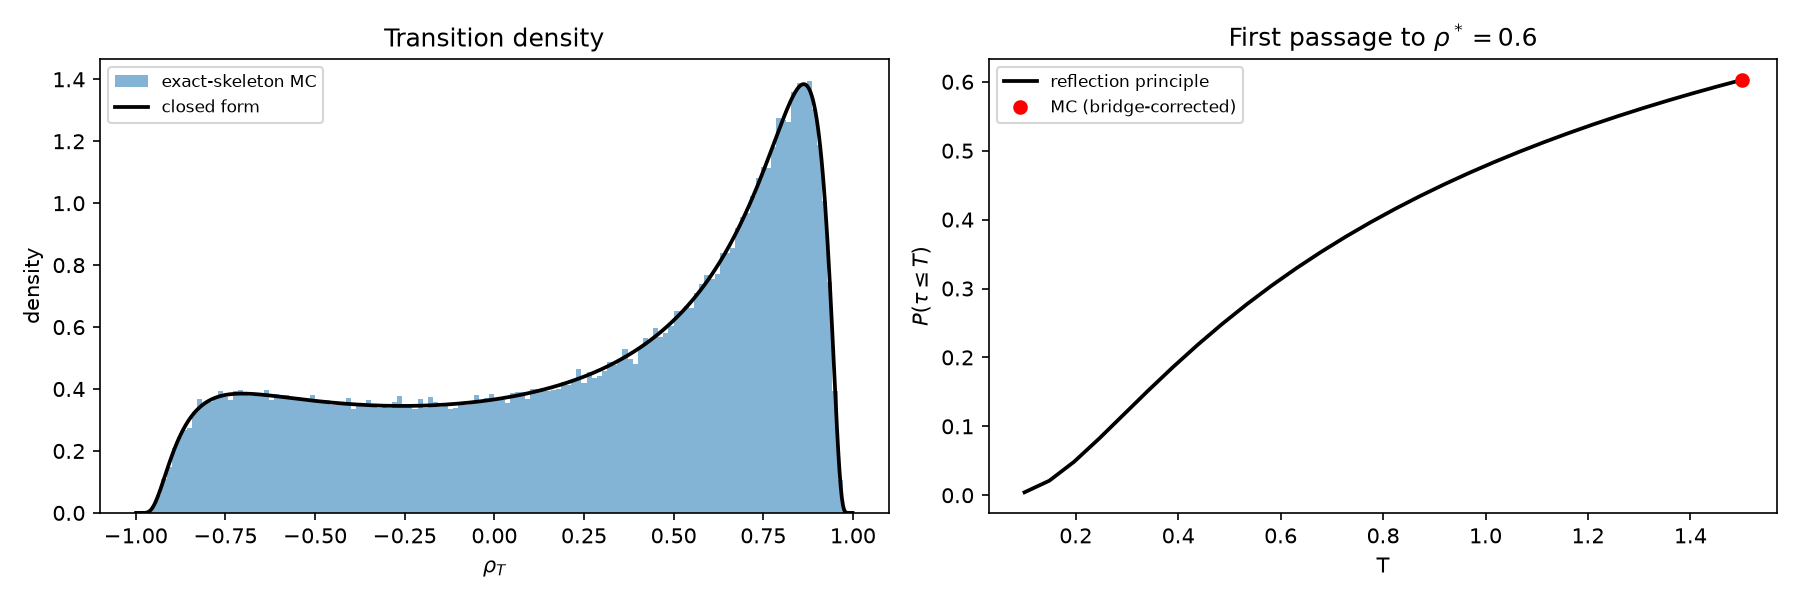
\includegraphics[keepaspectratio]{figures/correlation_kernels.png}}

}

\caption{\label{fig-kernels}Exact kernels of the bounded correlation
coordinate: transition density (left) and first-passage CDF (right),
closed forms against exact-skeleton Monte Carlo. Seed 20260727.}

\end{figure}%

\begin{proposition}[Measure-change
invariance]\protect\hypertarget{prp-measurechange}{}\label{prp-measurechange}

Under any equivalent martingale measure with constant market price of
correlation risk \(\lambda\), every law of this section and every price
of Section~\ref{sec-derivatives} holds verbatim with \(\mu\) replaced by
\(\mu^{\mathbb Q}=\mu+\sigma\lambda\).

\end{proposition}

\begin{proof}
Girsanov with constant \(\lambda\) maps drifted Brownian motion to
drifted Brownian motion (Girsanov 1960); the reflection principle and
the conjugate map see only the drift. ∎
\end{proof}

Since correlation is not a traded asset, the pricing measure is a choice
parameterized by \(\lambda\); Proposition~\ref{prp-measurechange} says
the exact-kernel class is \emph{closed} under that choice. The
correlation risk premium (Driessen et al. 2009) enters as one scalar
drift parameter, and price sensitivities to it are closed-form
comparative statics (no re-simulation).

\section{Correlation derivatives}\label{sec-derivatives}

All four products below are priced in terms of \(\Phi\) --- no series,
no transform inversion, no simulation. To our knowledge after the audit
of Section~\ref{sec-related}, these are the first closed-form prices for
correlation-barrier and correlation-range payoffs: the tractable
competitors cover European-type payoffs only, and barrier/touch
structures under stochastic correlation have approximations (Higgins
2014).

\begin{proposition}[Digital]\protect\hypertarget{prp-digital}{}\label{prp-digital}

\(V_{\mathrm{dig}}=e^{-rT}\Phi\!\big((\mu T-b)/(\sigma\sqrt T)\big)\),
paying \(\mathbf 1_{\{\rho_T\ge\rho^{*}\}}\) (any
\(\rho^{*}\in(-1,1)\)).

\end{proposition}

\begin{proposition}[One-touch paid at
expiry]\protect\hypertarget{prp-touch}{}\label{prp-touch}

\(V_{\mathrm{touch}}^{T}=e^{-rT}\,\mathbb P(\tau_\rho\le T)\) with
Theorem~\ref{thm-firstpassage} (a), paying
\(\mathbf 1_{\{\tau_\rho\le T\}}\) at \(T\).

\end{proposition}

\begin{theorem}[One-touch paid at hit --- a new closed
form]\protect\hypertarget{thm-touchhit}{}\label{thm-touchhit}

With \(\gamma=\sqrt{\mu^{2}+2r\sigma^{2}}\), \[
V_{\mathrm{touch}}^{\mathrm{hit}}
=
e^{-b(\gamma-\mu)/\sigma^{2}}
\Big[
\Phi\!\Big(\frac{\gamma T-b}{\sigma\sqrt T}\Big)
+
e^{2\gamma b/\sigma^{2}}
\Phi\!\Big(-\frac{\gamma T+b}{\sigma\sqrt T}\Big)
\Big],
\] paying \(1\) at \(\tau_\rho\) if \(\tau_\rho\le T\).

\end{theorem}

\begin{proof}
Completing the square,
\((b-\mu t)^{2}/(2\sigma^{2}t)+rt=(b-\gamma t)^{2}/(2\sigma^{2}t)
+b(\gamma-\mu)/\sigma^{2}\), so
\(e^{-rt}g_\tau^{(\mu)}(t)=e^{-b(\gamma-\mu)/\sigma^{2}}g_\tau^{(\gamma)}(t)\)
and the right side integrates as Theorem~\ref{thm-firstpassage} (a) with
drift \(\gamma\). ∎
\end{proof}

Consistency limits, enforced as unit tests: \(r\to0^{+}\) recovers
Proposition~\ref{prp-touch} undiscounted (both drift signs);
\(T\to\infty\) recovers the classical Laplace transform
\(e^{-b(\gamma-\mu)/\sigma^{2}}\); and
\(V_{\mathrm{touch}}^{\mathrm{hit}}\ge V_{\mathrm{touch}}^{T}\ge
V_{\mathrm{dig}}\).

\begin{proposition}[Discretely monitored range
accrual]\protect\hypertarget{prp-accrual}{}\label{prp-accrual}

For monitoring dates \(0<t_1<\dots<t_n=T\) and band
\((\rho_\ell,\rho_h)\), \[
V_{\mathrm{range}}
=
\sum_{i=1}^{n}e^{-rt_i}
\Big[
\Phi\!\Big(\frac{x(\rho_h)-x_0-\mu t_i}{\sigma\sqrt{t_i}}\Big)
-
\Phi\!\Big(\frac{x(\rho_\ell)-x_0-\mu t_i}{\sigma\sqrt{t_i}}\Big)
\Big],
\] paying \(\sum_i\mathbf 1_{\{\rho_\ell\le\rho_{t_i}\le\rho_h\}}\).
Either level may be \(\mp1\), recovering one-sided digitals.

\end{proposition}

Daily monitoring is how range accruals are written, so
Proposition~\ref{prp-accrual} is the practical product; the
\emph{continuous} corridor is the harder object and is solved in
Section~\ref{sec-corridor}.

The paper notebook reports all prices against bridge-corrected Monte
Carlo (within \(2\) standard errors), and plots the one-touch price
against the correlation risk premium \(\lambda\) of
Proposition~\ref{prp-measurechange} --- a closed-form comparative static
that the approximation literature cannot produce.

\section{Joint two-asset barriers: the variance-clock
reduction}\label{sec-reduction}

\subsection{Model}\label{model}

Two traded forward prices (martingales under the forward measure, so no
drifts appear), correlated through the bounded coordinate:

\[
dF_1=\sigma_1\,dW_1,\qquad
dF_2=\sigma_2\big(\rho_t\,dW_1+\sqrt{1-\rho_t^{2}}\,dW_2\big),
\]

with \(\rho_t=f(X_t)\) as before. \textbf{Structural assumption:} the
correlation driver \(W\) is independent of the asset drivers
\((W_1,W_2)\) --- the van Emmerich/Teng construction (Emmerich 2006;
Teng et al. 2016). The cost is the exclusion of leverage (correlation
does not respond to asset moves); see Section~\ref{sec-related}.

\begin{lemma}[Conditional
Gaussianity]\protect\hypertarget{lem-gaussian}{}\label{lem-gaussian}

Conditional on the correlation path \(\rho_{[0,T]}\), the pair
\((F_1,F_2)\) is Gaussian with deterministic covariance determined by
\(\rho_{[0,T]}\).

\end{lemma}

\begin{proof}
Itô integrals with (conditionally) deterministic integrands are
Gaussian; independence of \(W\) makes conditioning free. ∎
\end{proof}

\begin{theorem}[Deterministic variance
clock]\protect\hypertarget{thm-clock}{}\label{thm-clock}

Let \(Z=\alpha_1F_1+\alpha_2F_2\) (spread \(\alpha=(1,-1)\), basket
\(\alpha=(1,1)\)), \(z_0=\alpha_1F_{1,0}+\alpha_2F_{2,0}\).
Conditionally on \(\rho_{[0,T]}\), \[
Z_t\ \stackrel{\mathrm{law}}{=}\ z_0+B_{v(t)},\qquad
v(t)=\int_0^{t}q(\rho_s)\,ds,
\] \[
q(\rho)=\alpha_1^{2}\sigma_1^{2}+\alpha_2^{2}\sigma_2^{2}
+2\alpha_1\alpha_2\sigma_1\sigma_2\,\rho .
\]

\end{theorem}

\begin{proof}
\(Z\) is a continuous local martingale with quadratic variation
\(\int q(\rho_s)\,ds\), deterministic under conditioning; the
Dambis--Dubins--Schwarz theorem (Karatzas and Shreve 1991, Thm. 3.4.6)
applies. ∎
\end{proof}

\begin{corollary}[Scalar reduction of joint barrier
laws]\protect\hypertarget{cor-scalar}{}\label{cor-scalar}

For an upper barrier \(d>z_0\), \[
\mathbb P\!\Big(\sup_{t\le T}Z_t\ge d\ \Big|\ \rho_{[0,T]}\Big)
=
2\Big(1-\Phi\Big(\frac{d-z_0}{\sqrt{v(T;\rho)}}\Big)\Big),
\] and analogously for lower barriers and the joint law of
\((\sup Z,Z_T)\). Every claim measurable in the running extrema of \(Z\)
prices as \(e^{-rT}\mathbb E_\rho[g(v(T;\rho))]\) with \(g\) closed
form.

\end{corollary}

The three-driver pricing problem collapses to the law of one scalar
functional. The notebook verifies the theorem itself, not just its
consequences: a full three-driver simulation with bridge correction
matches the scalar reduction (z-scores \(-1.16\), \(+1.19\) at two step
sizes), with the reduction's standard error six times smaller --- an
effective-dimension reduction, not a relabeling.

\begin{corollary}[Sign theorem: spread
vs.~basket]\protect\hypertarget{cor-sign}{}\label{cor-sign}

The \(q\)-coefficient of \(\rho\) is
\(2\alpha_1\alpha_2\sigma_1\sigma_2\): negative for the spread, positive
for the basket. Correlation risk therefore moves spread-barrier and
basket-barrier prices in opposite directions, and constant-correlation
pricing misprices the two in opposite senses.

\end{corollary}

Figure~\ref{fig-mispricing} exhibits Corollary~\ref{cor-sign}: the gap
between stochastic- and constant-correlation one-touch prices has
opposite signs for spread and basket across the correlation-volatility
range. Since \(v\mapsto 2(1-\Phi(d/\sqrt v))\) changes convexity in
\(v\), the \emph{sign} of the Jensen gap is parameter-dependent and is
exhibited numerically rather than asserted as a theorem.

\begin{figure}[tbp]

\centering{

\pandocbounded{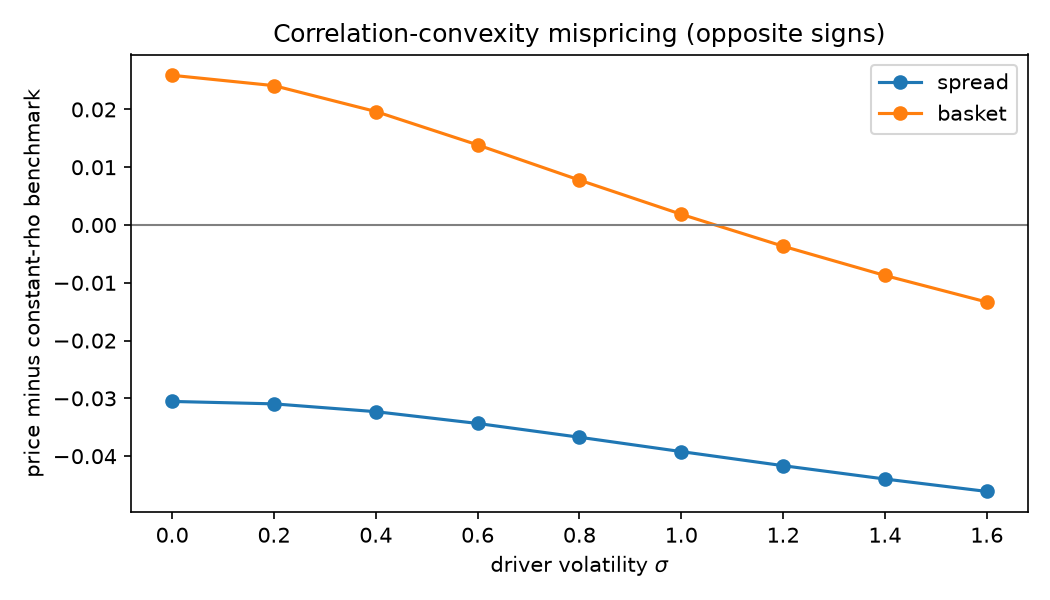
\includegraphics[keepaspectratio]{figures/spread_basket_mispricing.png}}

}

\caption{\label{fig-mispricing}Correlation-convexity mispricing:
stochastic-correlation one-touch price minus the constant-correlation
benchmark, for spread and basket barriers. Opposite signs, as
Corollary~\ref{cor-sign} requires. Seed 20260727.}

\end{figure}%

Working with forward prices is what makes Theorem~\ref{thm-clock} exact:
with nonzero drifts the running supremum depends on the whole variance
path, not only on \(v(T)\).

\section{The full clock law by Feynman--Kac}\label{sec-fk}

Corollary~\ref{cor-scalar} prices everything through the law of
\(v(T;\rho)=\beta T+\alpha A_T\) with
\(\beta=\alpha_1^{2}\sigma_1^{2}+\alpha_2^{2}\sigma_2^{2}\),
\(\alpha=2\alpha_1\alpha_2\sigma_1\sigma_2\) and
\(A_T=\int_0^T\rho_s\,ds\). The moments of \(A_T\) are deterministic
quadratures (Gauss--Hermite over the Gaussian factor, Gauss--Legendre
over the time simplex --- the naive square rule has a diagonal ridge;
the triangle-aware rule converges to machine precision). For the full
law:

\begin{theorem}[Bounded support Fourier
density]\protect\hypertarget{thm-fk}{}\label{thm-fk}

Let \(u(t,x)=\mathbb E_x[e^{i\xi\int_0^t f(X_s)\,ds}]\). Then \[
\partial_t u=\tfrac{\sigma^{2}}{2}u_{xx}+\mu u_x+i\xi f(x)\,u,\qquad
u(0,x)=1,
\] and \(\phi(\xi)=u(T,x_0)\) is the characteristic function of \(A_T\).
Since \(|f|<1\), the support of \(A_T\) is bounded in \((-T,T)\), and on
\([-T,T]\) the density is \[
p(a)=\frac{1}{2T}\sum_{k=-\infty}^{\infty}
\phi\!\Big(\frac{k\pi}{T}\Big)e^{-ik\pi a/T}.
\]

\end{theorem}

\begin{proof}
Feynman--Kac (Kac 1949) applies since the potential is bounded; the
Fourier representation is the standard series on a bounded interval. ∎
\end{proof}

One PDE solve per Fourier mode (Krylov time integration on a truncated
domain; the Dirichlet localization error is checked by doubling the
margin, cf. (Cont and Voltchkova 2005)). The price is

\[
V_{\mathrm{FK}}
=
e^{-rT}\int_{-T}^{T}g\big(\beta T+\alpha a\big)\,p_K(a)\,da ,
\]

with two monitored discretization errors (\(K\), grid). In all reported
configurations the deterministic price is statistically
indistinguishable from the exact-simulation benchmark (\(|z|<1\)); a
Gamma moment match on the quadrature moments remains as a fast screening
tool whose error against the resolvent price is measured per parameter
set (\(-5\times10^{-5}\) to \(-2\times10^{-3}\) across the
correlation-volatility range).

\section{Corridor occupation}\label{sec-corridor}

The continuous corridor pays on the occupation time
\(\mathcal O_T=\int_0^T\mathbf 1_{\{x_\ell\le X_t\le x_h\}}\,dt\) ---
exactly the occupation of the correlation band
\(\{\rho_\ell\le\rho_t\le\rho_h\}\). The plain corridor bond is linear
in \(\mathcal O_T\) and prices by quadrature of Gaussian probabilities
(an anchor, not a contribution); anything nonlinear --- a corridor
digital \(\mathbf 1_{\{\mathcal O_T\ge\kappa T\}}\) or call
\((\mathcal O_T/T-\kappa)^{+}\) --- needs the law.

The resolvent of Theorem~\ref{thm-fk} applies with potential
\(i\xi\mathbf 1_{[x_\ell,x_h]}\). Two structural facts drive the
computation:

\begin{proposition}[The never-exit
atom]\protect\hypertarget{prp-atom}{}\label{prp-atom}

A bounded corridor always has an atom at \(\mathcal O_T=T\) (never
exit), computable deterministically by the absorbing-boundary PDE on the
corridor; an unbounded corridor with drift has one in closed form from
Theorem~\ref{thm-firstpassage} (c). At the Fourier nodes
\(\xi_k=2\pi k/T\) the atom contributes its mass as a constant
(\(e^{i\xi_kT}=1\)), so it is subtracted from every mode and the Fourier
series represents only the continuous part.

\end{proposition}

\begin{theorem}[Arcsine
anchor]\protect\hypertarget{thm-arcsine}{}\label{thm-arcsine}

For \(\mu=0\), corridor \([0,\infty)\), \(x_0=0\), the occupation
fraction follows Lévy's arcsine law
\(\mathbb P(\mathcal O_T\le sT)=\frac{2}{\pi}\arcsin\sqrt s\) (Lévy
1939). The resolvent pipeline reproduces it: tail probabilities to
\(5\times10^{-4}\) (Figure~\ref{fig-arcsine}).

\end{theorem}

\begin{figure}[tbp]

\centering{

\pandocbounded{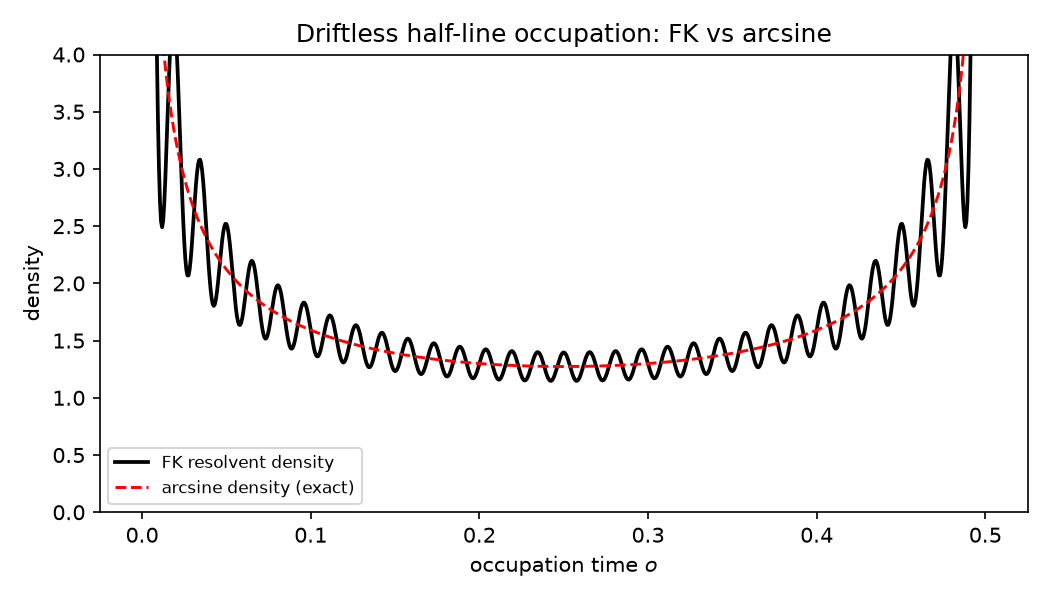
\includegraphics[keepaspectratio]{figures/corridor_arcsine.png}}

}

\caption{\label{fig-arcsine}Driftless half-line occupation: the FK
resolvent density against Lévy's exact arcsine density --- a
parameter-free, non-Gaussian benchmark. Seed 20260727.}

\end{figure}%

The notebook prices corridor digitals and calls against exact-skeleton
simulation; the residual gap (\(\sim7\times10^{-3}\)) is fully explained
by two identified opposite-sign biases (simulation overstates occupation
through bridge misses; Fourier truncation biases slightly downward), and
is recorded as such in the reproducibility material --- not reported as
statistical agreement.

\section{The OU driver and the stationarity--tractability
classification}\label{sec-ou}

Replace the driver by \(dX_t=\kappa(\bar x-X_t)\,dt+\sigma\,dW_t\),
\(\kappa>0\). The correlation coordinate inherits mean reversion and an
exact stationary density (Gaussian stationary law pushed through \(f\)),
answering the standard objection to non-stationary correlation models
(Teng et al. 2016).

\begin{theorem}[Stationarity--tractability
classification]\protect\hypertarget{thm-classification}{}\label{thm-classification}

For \(\rho_t=f(X_t)\) with \(X\) a scalar Gaussian factor:

{\def\LTcaptype{none} % do not increment counter
\begin{longtable}[]{@{}
  >{\raggedright\arraybackslash}p{(\linewidth - 6\tabcolsep) * \real{0.2500}}
  >{\raggedright\arraybackslash}p{(\linewidth - 6\tabcolsep) * \real{0.2500}}
  >{\raggedright\arraybackslash}p{(\linewidth - 6\tabcolsep) * \real{0.2500}}
  >{\raggedright\arraybackslash}p{(\linewidth - 6\tabcolsep) * \real{0.2500}}@{}}
\toprule\noalign{}
\begin{minipage}[b]{\linewidth}\raggedright
object
\end{minipage} & \begin{minipage}[b]{\linewidth}\raggedright
BM driver
\end{minipage} & \begin{minipage}[b]{\linewidth}\raggedright
OU driver
\end{minipage} & \begin{minipage}[b]{\linewidth}\raggedright
\end{minipage} \\
\midrule\noalign{}
\endhead
\bottomrule\noalign{}
\endlastfoot
stationarity & none & exact stationary density & \\
transition density & closed form & closed form & \\
digital / discrete accrual & closed form & closed form & \\
first-passage laws & closed form (reflection) & no closed form; FK
resolvent & \\
DDS variance clock & exact & exact (driver-agnostic) & \\
clock moments / full law & quadrature / FK & quadrature / FK (OU
generator) & \\
measure change, constant \(\lambda\) & \(\mu\to\mu+\sigma\lambda\) &
\(\bar x\to\bar x+\sigma\lambda/\kappa\) & \\
\end{longtable}
}

\end{theorem}

\begin{proof}
Static rows: OU transitions are Gaussian, and the conjugate map is
deterministic. First-passage row: OU hitting laws admit only series
representations (Ricciardi and Sato 1988; Alili et al. 2005); hitting
probabilities are path properties and the monotone map cannot repair
what the generator lacks. Clock rows: Theorem~\ref{thm-clock} conditions
on the realized path and never sees the generator. Measure-change row:
Girsanov with constant \(\lambda\) shifts the OU drift by a constant,
equivalently the long-run mean. ∎
\end{proof}

\begin{corollary}[The
frontier]\protect\hypertarget{cor-frontier}{}\label{cor-frontier}

In this model class, reflection-principle hitting laws and stationarity
are mutually exclusive: a Gaussian factor with a Gaussian stationary law
is not Brownian, and only Brownian motion has reflection-principle
hitting laws. Mean reversion is bought by surrendering closed-form
barrier laws to the resolvent; everything static and everything
clock-based survives.

\end{corollary}

The \(\kappa\to0^{+}\) degeneration anchors the implementation: every OU
formula reproduces its Brownian counterpart (density to
\(2\times10^{-7}\), occupation moments to \(6\times10^{-8}\)), and the
OU spread one-touch price from the resolvent matches exact OU simulation
(z \(=+0.92\)).

\section{Novelty boundary and related work}\label{sec-related}

\textbf{Established, not claimed.} Bounded correlation as a transform of
a Gaussian factor: van Emmerich (Emmerich 2006); tanh of a modified OU
with closed-form \emph{stationary} density and quanto pricing by
conditional Monte Carlo: Teng--Ehrhardt--Günther (Teng et al. 2016);
Jacobi correlation and Jacobi volatility with spectral methods (Ackerer
et al. 2018); circular correlation models with approximate likelihood
(Majumdar 2024); barrier/touch \emph{approximations} under stochastic
(spot--vol) correlation (Higgins 2014); the arctangent map as a
numerical compactification in finance (Duffie and Kan 1996; Hout and
Snoeijer 2021); arctangent-transformed Brownian motion as an exact SDE
example (Särkkä and Solin 2019); Bachelier pricing context
(Schachermayer and Teichmann 2008; Choi et al. 2022; CME Group 2020);
exact simulation beyond transform methods (Beskos and Roberts 2005). The
one-phase Euler chart itself is the companion paper (Complex--Itô
Random-Walk Research Project 2026).

\textbf{What the audit found open, and what is claimed here.} (i) Exact
finite-time kernels and reflection-principle first-passage laws for a
bounded correlation state (Theorem~\ref{thm-density},
Theorem~\ref{thm-firstpassage}) --- the competitors have stationary-only
densities, spectral densities, or approximate ones. (ii) Exact prices
for correlation-barrier and correlation-range payoffs, including the
pay-at-hit closed form of Theorem~\ref{thm-touchhit}
(Section~\ref{sec-derivatives}, Section~\ref{sec-corridor}) ---
previously approximation territory. (iii) The scalar variance-clock
reduction with its sign theorem (Theorem~\ref{thm-clock},
Corollary~\ref{cor-sign}) and the deterministic full clock law
(Theorem~\ref{thm-fk}). (iv) The stationarity--tractability
classification (Theorem~\ref{thm-classification}). Teng et al. (Teng et
al. 2016) considered and rejected an arctan-family correlation map for
its slow polynomial approach to \(\pm1\); we accept that cost explicitly
(it is the price of the reflection principle), and note the rejection
concerned a different member of the family (\((2/\pi)\arctan\) of the
factor, not \(\sin\circ\arctan\)), and was an estimation argument, not a
pricing one.

\textbf{Costs and exclusions, stated.} Under the Brownian driver the
coordinate is non-stationary (\(\rho_t\to\operatorname{sgn}\mu\) a.s.
for \(\mu\neq0\); recurrent extremes for \(\mu=0\)); the OU driver of
Section~\ref{sec-ou} answers this at the cost of
Corollary~\ref{cor-frontier}. Boundary approach is polynomial. The
reduction of Section~\ref{sec-reduction} excludes leverage
(\(W\perp(W_1,W_2)\)). Correlation is not traded; prices are conditional
on a chosen risk premium (Proposition~\ref{prp-measurechange}).
Estimation and calibration are deferred, though exact likelihoods are
immediate from Theorem~\ref{thm-density}.

\section{Conclusion}\label{sec-conclusion}

One bounded change of variables --- the sine of the one-phase Euler
phase --- carries Brownian exactness through every level of the
stochastic correlation problem: kernels, first passage, derivative
prices, joint barrier laws, occupation laws, and, with the OU driver, a
classified stationarity frontier. The framework's value is not a new
transform but the closed-form and deterministic content the transform
inherits from the reflection principle and the Feynman--Kac resolvent
--- content the tractable literature prices only by approximation.

\section*{Reproducibility}\label{sec-reproducibility}
\addcontentsline{toc}{section}{Reproducibility}

All numerical claims are produced by the companion notebook
(\texttt{notebooks/phase6\_correlation\_paper.ipynb}, seed 20260727,
runtime under one minute) from tested repository modules
(\texttt{phase6\_correlation.py}, \texttt{phase6\_joint.py},
\texttt{phase6\_fk.py}, \texttt{phase6\_corridor.py},
\texttt{phase6\_ou.py}; 77 unit tests). Key checks: transition density
and first-passage CDF vs.~exact-skeleton Monte Carlo
(Figure~\ref{fig-kernels}); derivative ordering
\(V_{\mathrm{dig}}\le V_{\mathrm{touch}}^{T}\le
V_{\mathrm{touch}}^{\mathrm{hit}}\); full three-driver vs.~scalar
reduction; FK price vs.~benchmark (\(|z|<1\)); arcsine tail to
\(5\times10^{-4}\); \(\kappa\to0^{+}\) anchors; OU price vs.~benchmark
(\(z=-0.14\)). Figures and machine-readable checks are in
\texttt{figures/} and \texttt{tables/}
(\texttt{verification\_summary.csv}).

\section*{References}\label{references}
\addcontentsline{toc}{section}{References}

\protect\phantomsection\label{refs}
\begin{CSLReferences}{1}{1}
\bibitem[\citeproctext]{ref-ackerer2018}
Ackerer, Damien, Damir Filipović, and Sergio Pulido. 2018. {``The Jacobi
Stochastic Volatility Model.''} \emph{Finance and Stochastics} 22 (3):
667--700. \url{https://doi.org/10.1007/s00780-018-0364-8}.

\bibitem[\citeproctext]{ref-alili2005}
Alili, Larbi, Pierre Patie, and Jesper L. Pedersen. 2005.
{``Representations of the First Hitting Time Density of an
{Ornstein--Uhlenbeck} Process.''} \emph{Stochastic Models} 21 (4):
967--80. \url{https://doi.org/10.1080/15326340500294702}.

\bibitem[\citeproctext]{ref-beskosroberts2005}
Beskos, Alexandros, and Gareth O. Roberts. 2005. {``Exact Simulation of
Diffusions.''} \emph{The Annals of Applied Probability} 15 (4):
2422--44. \url{https://doi.org/10.1214/105051605000000485}.

\bibitem[\citeproctext]{ref-borodinsalminen2002}
Borodin, Andrei N., and Paavo Salminen. 2002. \emph{Handbook of
{Brownian} Motion --- Facts and Formulae}. 2nd ed. Birkh{ä}user.
\url{https://doi.org/10.1007/978-3-0348-8163-0}.

\bibitem[\citeproctext]{ref-choi2022}
Choi, Jaehyuk, Minsuk Kwak, Chyng Wen Tee, and Yumeng Wang. 2022. {``A
{Black--Scholes} User's Guide to the {Bachelier} Model.''} \emph{Journal
of Futures Markets} 42 (5): 959--80.
\url{https://doi.org/10.1002/fut.22315}.

\bibitem[\citeproctext]{ref-cme2020}
CME Group. 2020. {``Clearing Advisory: {WTI} Crude Oil Options to Be
Revalued Using Bachelier Model.''}
\url{https://www.cmegroup.com/notices/clearing/2020/20090.html}.

\bibitem[\citeproctext]{ref-onephaseeuler2026}
Complex--Itô Random-Walk Research Project. 2026. \emph{One-Phase {Euler}
Coordinates for Affine {Brownian} Factors: Exact Classification, Pricing
Conjugacy, and Numerical Consequences}.

\bibitem[\citeproctext]{ref-contvoltchkova2005}
Cont, Rama, and Ekaterina Voltchkova. 2005. {``A Finite Difference
Scheme for Option Pricing in Jump Diffusion and Exponential l{é}vy
Models.''} \emph{SIAM Journal on Numerical Analysis} 43 (4): 1596--626.
\url{https://doi.org/10.1137/040613337}.

\bibitem[\citeproctext]{ref-driessen2009}
Driessen, Joost, Pascal J. Maenhout, and Grigory Vilkov. 2009. {``The
Price of Correlation Risk: Evidence from Equity Options.''} \emph{The
Journal of Finance} 64 (3): 1377--406.
\url{https://doi.org/10.1111/j.1540-6261.2009.01467.x}.

\bibitem[\citeproctext]{ref-duffiekan1996}
Duffie, Darrell, and Rui Kan. 1996. {``A Yield-Factor Model of Interest
Rates.''} \emph{Mathematical Finance} 6 (4): 379--406.
\url{https://doi.org/10.1111/j.1467-9965.1996.tb00123.x}.

\bibitem[\citeproctext]{ref-vanemmerich2006}
Emmerich, Christian van. 2006. \emph{Modelling Correlation as a
Stochastic Process}.

\bibitem[\citeproctext]{ref-girsanov1960}
Girsanov, Igor V. 1960. {``On Transforming a Certain Class of Stochastic
Processes by Absolutely Continuous Substitution of Measures.''}
\emph{Theory of Probability \& Its Applications} 5 (3): 285--301.
\url{https://doi.org/10.1137/1105027}.

\bibitem[\citeproctext]{ref-higgins2014}
Higgins, Mark. 2014. \emph{Stochastic Spot/Volatility Correlation in
Stochastic Volatility Models and Barrier Option Pricing}.

\bibitem[\citeproctext]{ref-inthoutsnoeijer2021}
Hout, Karel J. in 't, and Jacob Snoeijer. 2021. {``Numerical Valuation
of {American} Basket Options via Partial Differential Complementarity
Problems.''} \emph{Mathematics} 9 (13): 1498.
\url{https://doi.org/10.3390/math9131498}.

\bibitem[\citeproctext]{ref-kac1949}
Kac, Mark. 1949. {``On Distributions of Certain {Wiener} Functionals.''}
\emph{Transactions of the American Mathematical Society} 65 (1): 1--13.
\url{https://doi.org/10.2307/1990512}.

\bibitem[\citeproctext]{ref-karatzasshreve1991}
Karatzas, Ioannis, and Steven E. Shreve. 1991. \emph{Brownian Motion and
Stochastic Calculus}. 2nd ed. Springer.
\url{https://doi.org/10.1007/978-1-4612-0949-2}.

\bibitem[\citeproctext]{ref-levy1939}
Lévy, Paul. 1939. {``Sur Certains Processus Stochastiques
Homog{è}nes.''} \emph{Compositio Mathematica} 7: 283--339.

\bibitem[\citeproctext]{ref-majumdar2024}
Majumdar, Sourav. 2024. \emph{Diffusion on the Circle and a Stochastic
Correlation Model}.

\bibitem[\citeproctext]{ref-ricciardi1988}
Ricciardi, Luigi M., and Shunsuke Sato. 1988. {``First-Passage-Time
Density and Moments of the {Ornstein--Uhlenbeck} Process.''}
\emph{Journal of Applied Probability} 25 (1): 43--57.
\url{https://doi.org/10.2307/3214232}.

\bibitem[\citeproctext]{ref-sarkkasolin2019}
Särkkä, Simo, and Arno Solin. 2019. \emph{Applied Stochastic
Differential Equations}. Cambridge University Press.
\url{https://doi.org/10.1017/9781108186735}.

\bibitem[\citeproctext]{ref-schachermayerteichmann2008}
Schachermayer, Walter, and Josef Teichmann. 2008. {``How Close Are the
Option Pricing Formulas of {Bachelier} and {Black--Merton--Scholes}?''}
\emph{Mathematical Finance} 18 (1): 155--70.
\url{https://doi.org/10.1111/j.1467-9965.2007.00326.x}.

\bibitem[\citeproctext]{ref-teng2016}
Teng, Long, Matthias Ehrhardt, and Michael Günther. 2016. {``Modelling
Stochastic Correlation.''} \emph{Journal of Mathematics in Industry} 6
(1): 1--18. \url{https://doi.org/10.1186/s13362-016-0018-4}.

\end{CSLReferences}




\end{document}
